% =====================================================================
% N1 · The Recognition-Exposure Gap — ETRI Journal submission (Wiley NJD v5)
% ---------------------------------------------------------------------
% Double-blind review manuscript. Class = WileyNJDv5 with the AMS option
% (inline numeric [N] citations, ETRI's mandated style), STIX2COL two-column
% layout. Engine: XeLaTeX (STIX via fontspec) + xeCJK (Chinese seed queries).
% Citations are literal [N] markers in citation-appearance order; the numbered
% list lives in references_list.tex (auto-formatted from references_anon.bib).
% Anonymity: no real names/emails/affiliations; self-cites are "Anonymous"
% (refs [5],[20]); identity strings are absent from source and PDF metadata.
% Build: xelatex paper_etri ; xelatex
% =====================================================================
\documentclass[AMS,STIX2COL]{WileyNJDv5}

\usepackage{xeCJK}
\setCJKmainfont{Microsoft YaHei}
\usepackage{amsmath}
\usepackage{amssymb}
\usepackage{booktabs}
\usepackage{graphicx}
\usepackage{url}

\articletype{Article}
\received{DD Month YYYY}
\revised{DD Month YYYY}
\accepted{DD Month YYYY}
\journal{ETRI Journal}
\volume{00}
\copyyear{2026}
\startpage{1}

\begin{document}

\title{The Recognition-Exposure Gap: Why Upgrading Intent Detection Can Reduce Tool Availability in LLM Agents}
\author{Anonymous Author(s)}
\authormark{Anonymous Author(s)}
\titlemark{THE RECOGNITION-EXPOSURE GAP}
\address{Anonymous affiliation withheld for double-blind review}
\corres{Correspondence concerning this manuscript should be directed to the handling editor as part of the double-blind review process.}

\abstract[Abstract]{Tool-rich LLM agents gate tool visibility by intent-detection confidence, exposing a narrow set when confident, a broad set otherwise---assumed monotone in detector quality. We report a counterintuitive failure. In a production desktop agent (WeClaw, 125 tools), an LLM detector raised recommendation accuracy to 98.2\% (491/500 queries, ground truth fixed by construction) yet \emph{lowered} exposure coverage to 42.2\%: in 56.2\% of cases the correct tool was named but never entered the function-calling schema. We name this the \textbf{Recognition-Exposure Gap}: two decoupled stages---confidence-to-tier mapping and exposure-set construction---that a confidence-shifting upgrade leaves desynchronized, dropping recognized tools. A deterministic replay and a live run quantify the cost: 788 failed round-trips, 499 escalations, 3.7$\times$ exposure inflation, and 2.6$\times$ per-query latency. A zero-training fix that merges recognized tools into the exposure set closes the gap (reachability 42.2\%$\rightarrow$98.4\%) and lowers exposure. The condition is defined detector- and framework-independently; we support this with blind second annotation ($\kappa=0.987$), three-detector replication, and open-source reproduction.}

\keywords{tool exposure; LLM agents; function calling; intent detection; agent harness}

\maketitle

% =====================================================================
% N1 · The Recognition-Exposure Gap — ETRI Journal submission body
% ---------------------------------------------------------------------
% Double-blind manuscript body, \input by paper_etri.tex (Wiley NJD v5,
% AMS + STIX2COL, compiled with XeLaTeX). Citations are literal [N]
% markers in appearance order; the numbered list lives in
% references_list.tex. Prose was LaTeX-ified from the internal draft:
% symbols -> math, %/_ escaped.
% =====================================================================



\section{Introduction}
\label{sec:intro}

As LLM agents gain access to hundreds of tools, exposing all of them at once becomes prohibitively expensive: full-schema prompts inflate token cost, latency, and selection error. A common remedy is \textbf{confidence-tiered exposure}---the harness runs an intent detector over the user's request, maps the detector's confidence to a visibility tier (a narrow \emph{recommended} set at high confidence, a broader \emph{extended} or \emph{full} set otherwise), and exposes only that tier's tools to the model's function-calling interface. This design is explicitly ``confidence-gated'' in recent systems~[1,2] and underlies a broad ``route before reasoning'' family~[3,4].

The design carries an implicit assumption: \textbf{exposure quality is monotone in detector quality}. If the intent detector improves---say, from keyword rules to an LLM---the correct tool should become \emph{more} reachable, not less. However, this paper shows the assumption can fail silently. In WeClaw~[5], a production daily-use desktop agent with 125 registered tools, we upgraded the intent detector from a rule-based matcher to an LLM-based classifier.\footnote{\textbf{LLM use disclosure.} A large language model was used to assist with literature survey, drafting, and language editing of this manuscript. All scientific claims, the failure-mode analysis, the experimental design, the production code paths under study, and the reported results are the intellectual product of the human authors, who take full responsibility for the content. No LLM is listed as an author.} The upgrade behaved essentially as intended at the recognition stage: on a 500-query set of colloquial, ambiguous user queries (25 tools, ground truth fixed \emph{by construction}), the LLM recommended the correct tool in \textbf{98.2\%} of cases (491/500; Wilson 95\% CI [96.6, 99.1]). Yet the fraction of those queries for which the recommended tool actually appeared in the function-calling exposure set was only \textbf{42.2\% (211/500)} [37.9, 46.6]. In the remaining \textbf{56.2\%} (281/500) [51.8, 60.5], the agent had correctly recognized what the user needed and then failed to make the corresponding tool callable. We call this divergence the \textbf{Recognition-Exposure Gap}.

The cause is structural, not a coding mistake. Confidence-tiered exposure is implemented as two stages: \textbf{Stage A} maps detector confidence to a tier; \textbf{Stage B} constructs the concrete tool set for that tier. When the detector is upgraded, its confidence distribution shifts---in our case the LLM returns a fixed high confidence (0.9) on success, collapsing every ambiguous query into the \emph{narrowest} tier. Stage B, however, still builds that tier's tool set from the \emph{rule-driven} intent-to-tool mapping, which is empty for colloquial queries; the LLM's recommended tools are recorded as annotations and prompt hints but are \textbf{not merged into the exposure set}. The two stages are decoupled: a recognition improvement changes Stage A's output without propagating to Stage B's construction, so correctly recognized tools are silently dropped. Consequently, recognition accuracy---the metric everyone watches---cannot see this.

Moreover, the gap is not a benign offline curiosity. We quantify its runtime consequence two ways. A \emph{deterministic replay} faithfully drives the production failure-escalation ladder (a tool call that cannot be resolved triggers \texttt{report\_failure}, which after a threshold escalates the tier and re-exposes tools): across the 281 gap queries it incurs \textbf{788 failed round-trips} and \textbf{499 tier escalations}, inflating the mean exposed tool set from 12.1 at the first round to \textbf{44.7} at the final tier. A separate \emph{real end-to-end run}---every round genuinely calling the LLM and measuring wall-clock---confirms the same asymmetry at true cost: mean per-query latency \textbf{11.2\,s before $\rightarrow$ 4.3\,s after} (a \textbf{2.6$\times$} reduction), with mean round-trips 2.58 $\rightarrow$ 1.03. The agent eventually does the right thing---but late, and at a cost. We then show a \textbf{zero-training co-design fix}: merging recognized tools into the exposure set at construction time closes the gap (first-attempt reachability 42.2\% $\rightarrow$ 98.4\% live, 100\% under deterministic replay; failed round-trips and escalations $\rightarrow$ 0) and, because it avoids escalation to the broad tier, keeps the exposed set near its first-round size (mean 12.1 $\rightarrow$ 13.2 offline) rather than inflating it to 44.7.

\textbf{Contributions.} (1)~We \emph{name} the Recognition-Exposure Gap, a failure mode localized at the \emph{interface between two harness modules} rather than in the model's representations, and show it occurs even when recognition is $\sim$98\% correct on a 500-query set. (2)~We contribute a \emph{reusable coverage-vs-recognition audit method}: a black-box, three-probe protocol (offline counterfactual, deterministic escalation replay, and live end-to-end run) that measures the divergence between what a harness recognizes and what it actually exposes, applicable to any confidence-tiered exposure system. Using it, we quantify the gap's runtime cost---a deterministic replay of the production escalation engine (reproducing round2's 42.2\% coverage / 56.2\% gap) and an independent live run that calls the LLM every round and measures wall-clock latency. (3)~We give a zero-training co-design fix---an \emph{existence proof that the gap is closable at construction time} (first-attempt reachability 42.2\% $\rightarrow$ 98.4\% live, 100\% under deterministic replay)---and abstract a failure condition that is \emph{defined} detector- and framework-independently, substantiating it with a second-annotator agreement study (Cohen's $\kappa=0.987$), replication across three heterogeneous LLM intent detectors, and a reference reproduction of the same two-stage decoupling inside three common open-source exposure strategies. We position the result as, to our knowledge, the first quantified tool-exposure instance of the model--harness ``coupling bottleneck''~[6].

\section{Background: Confidence-Tiered Tool Exposure}
\label{sec:background}

\textbf{System.} WeClaw~[5] is an open-source desktop LLM agent for daily personal use, with 125 registered tools spanning shell, file, screen, and search (the four \emph{core} tools always exposed), plus $\sim$23 \emph{extended} tools (browser, clipboard, calculator, datetime, notification, app control, stock query, enterprise lookup, and others) and a long tail of domain tools.

\textbf{Tiered exposure.} A \texttt{ToolExposureEngine} maps an intent result to a visibility tier by confidence: confidence $\geq$ 0.8 $\rightarrow$ \texttt{RECOMMENDED} (narrowest), $\geq$ 0.5 $\rightarrow$ \texttt{EXTENDED}, else \texttt{FULL}. For each tier it constructs a concrete tool-name set: \texttt{RECOMMENDED} = core tools $\cup$ intent-to-tool mapping for the recognized intents $\cup$ a capability-info tool; \texttt{EXTENDED} adds the $\sim$23 extended tools; \texttt{FULL} either exposes all registered tools or, under a retrieval-based fallback, a lexical Top-K union with a conservative floor. The constructed set is resolved for dependencies and is rendered into function-calling schemas---the hard boundary of what the model can call.

\textbf{Failure escalation.} The engine maintains a per-task consecutive-failure counter. When a tool call cannot be resolved, \texttt{report\_failure} increments it; once it reaches a threshold (2 in production), \texttt{\_upgrade\_tier} widens the tier (\texttt{RECOMMENDED} $\rightarrow$ \texttt{EXTENDED} $\rightarrow$ \texttt{FULL} $\rightarrow$ unbounded) and the next attempt re-exposes tools at the wider tier. This ladder is the runtime safety net that recovers from an under-exposed first attempt---at the cost of extra round-trips.

\textbf{The two stages.} We separate, for analysis, \textbf{Stage A} (confidence $\rightarrow$ tier) from \textbf{Stage B} (tier $\rightarrow$ tool set construction). The Recognition-Exposure Gap arises precisely because these stages are decoupled: the detector's recommended tools influence Stage A's confidence but, absent an explicit merge, do not influence Stage B's construction.

\section{The Recognition-Exposure Gap}
\label{sec:gap}

Let a query carry a ground-truth target tool \texttt{ref} (the tool a correct assistant should call). Define two booleans produced by \emph{different} pipeline stages:
\begin{itemize}
  \item \texttt{rec\_hit} = the intent detector \textbf{recommended} \texttt{ref} (Stage A / recognition);
  \item \texttt{exposed} = \texttt{ref} $\in$ the \textbf{function-calling exposure set} (Stage B / construction).
\end{itemize}

The \textbf{Recognition-Exposure Gap} is the event $\texttt{rec\_hit} \wedge \neg\,\texttt{exposed}$: the agent recognized the needed tool but did not make it callable. $P(\texttt{rec\_hit})$ is reported by recognition accuracy and $P(\texttt{exposed})$ by exposure coverage; the gap is their divergence. As a result, the gap is invisible to standard evaluations, which report only recognition accuracy.

\textbf{General failure condition.} The gap arises whenever a harness combines (a)~\textbf{confidence-tiered exposure}, where a detector-confidence shift can move queries into a narrower tier, with (b)~\textbf{decoupled recommended-tool injection}, where the detector's recommended tools are not merged into the tier's constructed set. Under (a)+(b), \emph{any} detector upgrade that raises confidence---paradoxically, an improvement---can push ambiguous queries into the narrowest tier while the recommended tools remain outside it. Moreover, the condition is \emph{defined} detector-independently (rules, LLM, or hybrid) and framework-independently (any harness with the two-stage structure). We verify it on a production LLM detector, replicate the recognition stage across three heterogeneous LLM detectors, isolate the mechanism via deterministic replay, and reproduce the same decoupling inside three common open-source exposure strategies (Section~\ref{sec:exp}).

\begin{figure*}[t]
\begin{center}
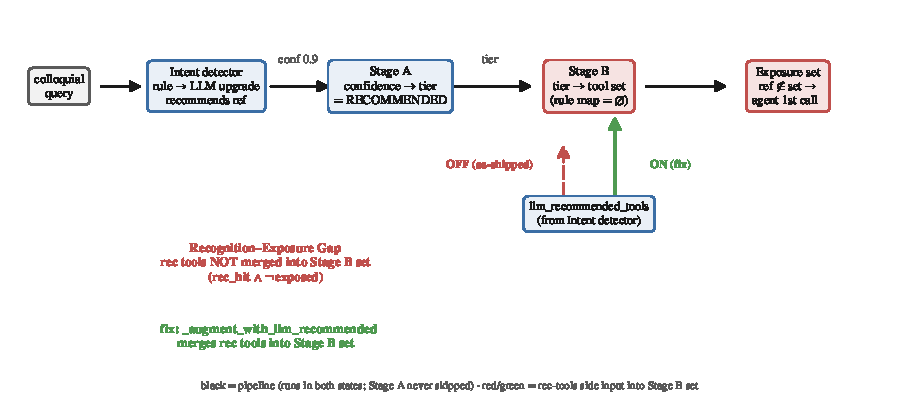
\includegraphics[width=0.8\textwidth]{figures/fig1_mechanism.pdf}
\end{center}
\caption{Mechanism of the Recognition-Exposure Gap. The intent detector's recommended tools drive Stage A's confidence (solid arrow) but are not merged into Stage B's tool-set construction (dashed, $\times$), so a correctly recognized tool never enters the function-calling exposure set; the zero-training fix (green) reconnects the two decoupled stages.}
\label{fig:mechanism}
\end{figure*}

\textbf{Terminology.} We use \emph{tool exposure} in its \textbf{capability} sense---the set of tools a harness makes visible/callable to the model---strictly distinct from \emph{data over-exposure} in the privacy sense~[7], which concerns an agent transmitting sensitive data beyond functional necessity. The two are in fact opposite failure directions of the same interface: over-exposure risks privacy, \textbf{under-exposure} (this work) risks capability. We return to this framing in Section~\ref{sec:related}.

\section{Method: Measuring and Closing the Gap}
\label{sec:method}

\textbf{4.1 Offline counterfactual (round2).} We reproduce the production LLM-intent path: for each query, an LLM classifier returns an intent result with recommended tools, and whether \texttt{ref} is in the exposure set the engine actually constructs is checked. This yields \texttt{rec\_hit}, \texttt{exposed}, and thus the gap without executing tool calls---the fast, first-order measurement. We run it on a 500-query set (25 tools, up to 20 queries per tool, with the ground-truth \texttt{ref} fixed \emph{by construction} from each query's seeded intent); every reported rate carries a Wilson 95\% confidence interval.

\textbf{4.2 Deterministic escalation-ladder replay (round3).} In order to measure the gap's \emph{runtime} consequence, we faithfully replay the escalation ladder. For each query we drive the real production code path (\texttt{\_determine\_tier} $\rightarrow$ \texttt{\_get\_tool\_names\_for\_tier} $\rightarrow$ dependency resolution) round by round: if \texttt{ref} $\notin$ exposed set, a failed round-trip is recorded (the semantics of an unresolvable first function call) and \texttt{report\_failure} is called, which escalates the tier once the threshold is reached; tools are exposed again and the round is repeated until \texttt{ref} becomes reachable (recovery) or the ladder tops out. In order to eliminate API nondeterminism and cost, round3 is a \textbf{deterministic replay}: it injects round2's measured recommendation outcome (\texttt{llm\_recommended\_tools = [ref]}) rather than re-calling the LLM, while exposure construction and escalation are performed through the unmodified production engine. We run two arms on the same queries: \textbf{before} (merge off, the pre-fix behavior) and \textbf{after} (merge on, the fix).

\textbf{4.3 Zero-training co-design fix.} The fix merges recognized tools into the exposure set at construction time: \texttt{\_augment\_with\_llm\_recommended} inserts \texttt{llm\_recommended\_tools} into both the \texttt{FULL}-fallback and non-\texttt{FULL} return points of Stage B, under four guards (config gate; known-tool filtering against the registry; forbidden-tool precedence; a \texttt{max\_merge} cap of 8). In other words, the fix simply connects Stage A's output to Stage B's construction: no model is trained and no threshold is retuned.

\textbf{4.4 Real end-to-end run (live).} Because the deterministic replay (4.2) fixes recognition and uses a per-round-trip latency proxy, we separately run a \emph{live} variant that removes both idealizations: on the same 500 queries, every round makes a genuine function-calling request to the production LLM (\texttt{deepseek-v4-flash}) against the currently exposed schemas, and we measure true wall-clock latency. The model's own tool choice (not an injected \texttt{ref}) drives whether a round resolves; a miss triggers the real \texttt{report\_failure}/\texttt{\_upgrade\_tier} ladder exactly as in production. To make the cost measure independent of client-side concurrency, we report the \emph{accumulated per-round-trip model latency} (sum of measured round-trip times per query), not wall-clock queueing time. This confirms the replay's before/after asymmetry under real API nondeterminism and real latency.

\textbf{4.5 Validation protocols.} Three protocols stress-test the headline claim. (i)~\emph{Blind second annotation}: because \texttt{ref} is fixed by construction, we cross-check it against an independent, different-provider LLM annotator (\texttt{qwen-max}) that, from the query and tool list alone, picks the tool a correct assistant should call; we report raw agreement and Cohen's $\kappa$. (ii)~\emph{Multi-detector replication}: we re-run the recognition stage with two additional different-provider detectors (\texttt{qwen-max}, \texttt{glm-5}) on a stratified subsample; since the merge-off exposure set is fixed by the rule intent (detector-independent), any cross-detector difference is attributable to recognition alone. (iii)~\emph{Reference reproduction on open-source strategies}: we implement three common exposure strategies---an intent-router with a static allow-list, an all-tools full-bind, and a Top-K tool retriever---under the same recognition signal, with and without the merge fix, to test whether the gap is a property of the two-stage architecture rather than of WeClaw specifically.

\section{Experiments}
\label{sec:exp}

\textbf{5.1 Setup.} The evaluation set is 500 colloquial, ambiguous Chinese queries spanning 25 tools (up to 20 per tool; e.g., ``现在几点了'' / ``what time is it now'' $\rightarrow$ \texttt{datetime\_tool}, ``帮我算个数'' / ``help me do a calculation'' $\rightarrow$ \texttt{calculator}, ``弹个通知提醒我'' / ``pop me a notification'' $\rightarrow$ \texttt{notify}); each query's ground-truth \texttt{ref} is fixed \emph{by construction} from its seeded intent, so the label is independent of any detector. The intent LLM is \texttt{deepseek-v4-flash}, which on success returns confidence 0.9 (collapsing queries into \texttt{RECOMMENDED}). Escalation threshold = 2 (production value); for the deterministic replay the per-failed-round-trip cost proxy is 1,950\,ms (a lower bound, since a real round-trip also includes tool execution and second-pass generation), while the live run (Section~5.6) measures true wall-clock ($\sim$4.16\,s mean per round-trip). Registered tools = 125. All rates carry Wilson 95\% confidence intervals.

\textbf{5.2 Offline counterfactual (round2).} Table~\ref{tab:offline} reports the recognition/exposure divergence. The LLM recommends the correct tool in 98.2\% of cases. However, fewer than half of those recommended tools are actually exposed; merging recognized tools lifts counterfactual coverage to 98.4\%.

\begin{table}[t]
\caption{Offline counterfactual measurement (round2), LLM intent detection, 500 queries whose ground-truth \texttt{ref} is fixed by construction; 95\% Wilson CIs in brackets. The tier collapse and exposure drop are deterministic code-path consequences; the 98.2\% recognition hit is a real LLM measurement, and blind second annotation agrees at $\kappa=0.987$ (Section~5.7). Exposure sizes are the offline constructed set (cf.\ Table~\ref{tab:execution}'s dependency-resolved first-attempt sizes).}
\label{tab:offline}
\begin{center}
\footnotesize
\begin{tabular}{ll}
\toprule
\textbf{Metric} & \textbf{Value} \\
\midrule
LLM recommendation hit (\texttt{rec\_hit}) & \textbf{98.2\%} (491/500) [96.6, 99.1] \\
Real exposure coverage (\texttt{exposed}) & \textbf{42.2\%} (211/500) [37.9, 46.6] \\
\textbf{Recognition-Exposure Gap} & \textbf{56.2\%} (281/500) [51.8, 60.5] \\
Coverage \emph{with} merge fix & \textbf{98.4\%} (492/500) [96.9, 99.2] \\
Mean exposure size (before $\rightarrow$ after) & 12.1 $\rightarrow$ 13.2 tools \\
\bottomrule
\end{tabular}
\end{center}
\end{table}

\begin{figure}[t]
\begin{center}
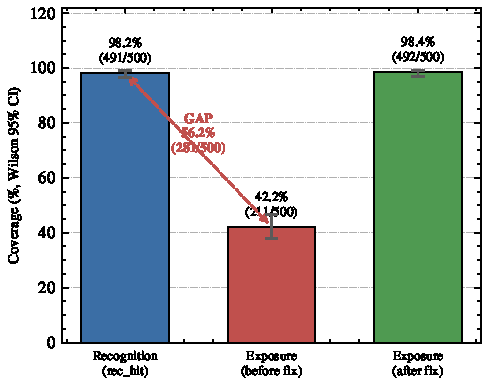
\includegraphics[width=\linewidth]{figures/fig2_recognition_exposure_gap.pdf}
\end{center}
\caption{Recognition vs.\ exposure coverage (round2, 500 queries with a ground-truth tool fixed by construction; error bars are Wilson 95\% CIs). The LLM recommends the correct tool in 98.2\% of cases, yet only 42.2\% of those tools are actually exposed (gap 56.2\%); merging recognized tools into the exposure set restores 98.4\% coverage.}
\label{fig:recog_expo}
\end{figure}

\textbf{5.3 Deterministic replay results (round3).} Table~\ref{tab:execution} contrasts the two arms under deterministic replay. Before the fix, only 42.2\% of queries can call the recommended tool on the first attempt; the other 57.8\% must detour through the escalation ladder, and all of them do eventually recover. In aggregate the detour costs \textbf{788 failed round-trips} and \textbf{499 tier escalations} across the 281 gap queries, inflating the mean exposed set from 12.1 (first round) to 44.7 at the final tier and accumulating a 1,536,600\,ms ($\approx$5.5\,s per gap query) latency lower bound. After the fix, first-attempt reachability is 100\%, with zero failed round-trips, zero escalations, and zero added latency; mean exposure stays at 12.7 instead of escalating to 44.7, because no query is forced up to the broad tier (the fix adds only the recognized tool at the first attempt but avoids the blow-up).

\begin{table}[t]
\caption{Deterministic escalation-ladder replay (round3), before/after arms on the same 500 queries (escalation threshold 2). First-attempt sizes are dependency-resolved, hence 12.1 matching Table~\ref{tab:offline}'s offline first-round mean. The after-arm merges only the ground-truth \texttt{ref} per query, so its exposure (12.7) is a lower bound; with the full recommended list the offline mean is 13.2 (Table~\ref{tab:offline}).}
\label{tab:execution}
\begin{center}
\footnotesize
\begin{tabular}{lcc}
\toprule
\textbf{Metric} & \textbf{before (merge off)} & \textbf{after (merge on)} \\
\midrule
First-attempt reachability & \textbf{42.2\%} [37.9, 46.6] & \textbf{100\%} [99.2, 100] \\
Need-detour rate & 57.8\% [53.4, 62.1] & \textbf{0\%} \\
Recovery after detour & 100\% (289/289) & n/a \\
Failed round-trips (total) & \textbf{788} & \textbf{0} \\
Tier escalations (total) & \textbf{499} & \textbf{0} \\
Mean first-round exposure & 12.1 & 12.7 \\
Mean final-tier exposure & \textbf{44.7} & 12.7 \\
Extra latency LB (cumulative) & \textbf{$\approx$5.5\,s/query} & \textbf{0} \\
\bottomrule
\end{tabular}
\end{center}
\end{table}

\begin{figure*}[t]
\begin{center}
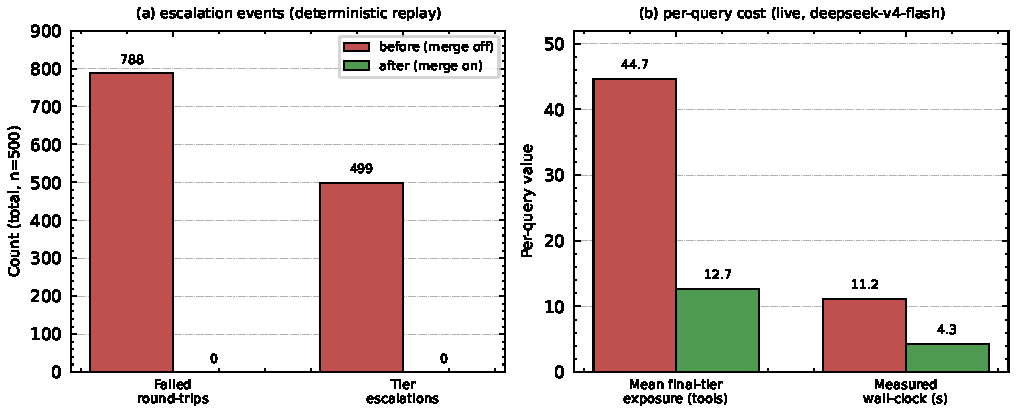
\includegraphics[width=0.95\textwidth]{figures/fig3_execution_cost.pdf}
\end{center}
\caption{Runtime cost, before vs.\ after the fix. (a)~Deterministic replay over 500 queries: the gap incurs 788 failed round-trips and 499 tier escalations, both driven to 0 by the fix. (b)~Per-query cost: mean final-tier exposure inflates from 12.1 to 44.7 tools under the ladder (12.7 after the fix), and a real end-to-end run measures mean accumulated latency 11.2\,s before vs.\ 4.3\,s after (2.6$\times$).}
\label{fig:exec_cost}
\end{figure*}

Table~\ref{tab:chains} shows representative trigger chains from the before arm. The pattern is uniform: two failed attempts inside the \texttt{RECOMMENDED} tier (the recommended tool is absent), then one escalation to \texttt{EXTENDED}, where the tool finally appears. Control queries whose \texttt{ref} is a core/always-resident tool (\texttt{file}, \texttt{search}, capability-info) reach on the first attempt in both arms, confirming the chain does not over-report.

\begin{table*}[t]
\caption{Representative before-arm trigger chains (rt = round-trip; tier, $|$exposed$|$, whether \texttt{ref} is reachable).}
\label{tab:chains}
\begin{center}
\small
\begin{tabular}{@{}p{2.15in}p{1.45in}p{2.75in}@{}}
\toprule
\textbf{Query (zh / en gloss)} & \textbf{\texttt{ref}} & \textbf{Trajectory} \\
\midrule
现在几点了 / ``what time is it now'' & \texttt{datetime\_tool} & rt1[REC, 5, $\times$] $\rightarrow$ rt2[REC, 5, $\times$] $\rightarrow$ rt3[EXT, 31, $\checkmark$] \\
帮我算个数 / ``help me do a calculation'' & \texttt{calculator} & rt1[REC, 5, $\times$] $\rightarrow$ rt2[REC, 5, $\times$] $\rightarrow$ rt3[EXT, 31, $\checkmark$] \\
弹个通知提醒我 / ``pop me a notification'' & \texttt{notify} & rt1[REC, 11, $\times$] $\rightarrow$ rt2[REC, 11, $\times$] $\rightarrow$ rt3[EXT, 34, $\checkmark$] \\
查下这家公司背景 / ``look up this company's background'' & \texttt{enterprise\_query} & rt1[REC, 5, $\times$] $\rightarrow$ rt2[REC, 5, $\times$] $\rightarrow$ rt3[EXT, 31, $\checkmark$] \\
处理个文档 / ``handle a document'' \emph{(control)} & \texttt{file} (core) & rt1[REC, 8, $\checkmark$] --- reachable first attempt in both arms \\
搜点资料 / ``search some material'' \emph{(control)} & \texttt{search} (core) & rt1[REC, 5, $\checkmark$] --- reachable first attempt in both arms \\
\bottomrule
\end{tabular}
\end{center}
\end{table*}

\begin{figure*}[t]
\begin{center}
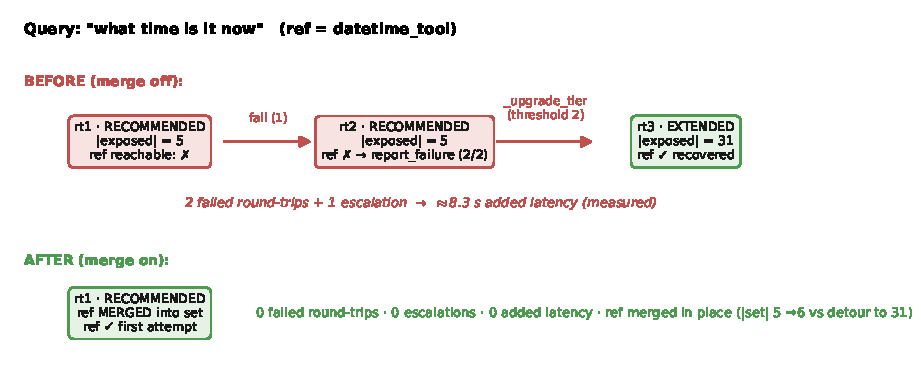
\includegraphics[width=0.8\textwidth]{figures/fig4_trigger_chain.pdf}
\end{center}
\caption{Representative before-arm trigger chain for ``what time is it now'' (\texttt{ref} = \texttt{datetime\_tool}): two failed round-trips inside the \texttt{RECOMMENDED} tier ($|$exposed$|$ = 5, \texttt{ref} absent), then one escalation to \texttt{EXTENDED} ($|$exposed$|$ = 31) where the tool finally becomes reachable; after the fix the tool is reachable on the first attempt.}
\label{fig:trigger_chain}
\end{figure*}

\textbf{5.4 Floor ablation (round0/round1).} A separate ablation (Figure~\ref{fig:floor}) isolates the extended-tool floor of the \texttt{FULL} tier. Removing the floor causes \textbf{50\%} of ambiguous queries to miss a high-frequency tool on the first attempt in the \texttt{FULL} tier (e.g., datetime, calculator, browser); back-filling colloquial keywords into tool descriptions drops the escalation trigger rate from \textbf{50\% $\rightarrow$ 0\%} and retrieval zero-hits from 4/20 $\rightarrow$ 1/20. Thus, this confirms the gap's mechanism is about \emph{which tools enter the constructed set}, and that the failure condition is not specific to the LLM detector---any confidence distribution that lands ambiguous queries in a narrow tier without the recommended tools reproduces it.

\begin{figure}[t]
\begin{center}
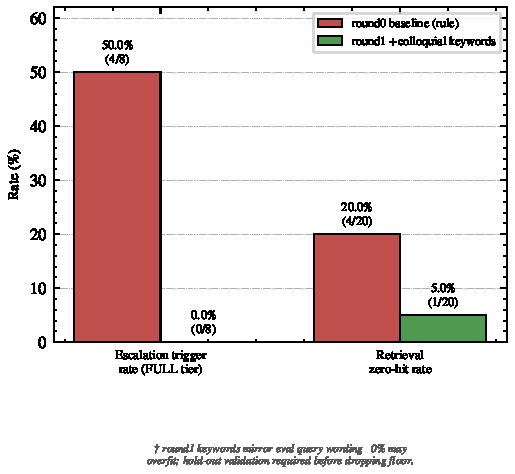
\includegraphics[width=\linewidth]{figures/fig5_floor_ablation.pdf}
\end{center}
\caption{\textbf{(supplementary)} FULL-tier floor ablation (round0 vs.\ round1, rule-based intent). Removing the extended-tool floor makes 50\% of ambiguous FULL-tier queries escalate (4/8) and leaves a 20\% lexical-retrieval zero-hit rate (4/20); back-filling colloquial keywords into tool descriptions drops both to 0\% (0/8) and 5\% (1/20). The floor-removal result is wording-independent and isolates the mechanism (which tools enter the constructed set); the keyword back-fill is an upper bound whose overlap with the evaluation wording is noted in the Limitations.}
\label{fig:floor}
\end{figure}

\textbf{5.5 Cross-validation.} The three execution-side methods agree: round3's deterministic first-attempt reachability (42.2\% before / 100\% after) matches round2's real exposure coverage (42.2\%) and gap (56.2\%), and the live end-to-end run (Section~5.6) independently reproduces the same 42.2\% first-attempt split under genuine per-round LLM calls. The replay and live probes re-derive exposure and escalation through the unmodified production engine while taking round2's measured recognition outcome as a given input (the replay does not re-call the LLM; the live run does), so they are not statistically independent at the recognition stage. Nevertheless, they independently confirm the exposure-construction and escalation behavior, strengthening confidence that the gap is a real property of the pipeline rather than an artifact of either probe.

\textbf{5.6 Real end-to-end run (live).} Table~\ref{tab:live} reports the live arm, in which every round issues a genuine \texttt{deepseek-v4-flash} function-calling request against the currently exposed schemas and wall-clock latency is measured. The first-attempt split (42.2\% before / 98.4\% after) reproduces the offline coverage, and both arms eventually reach 100\%. The fix's effect on cost is direct: mean round-trips per query fall from 2.58 to 1.03 and mean accumulated model latency from 11.2\,s to 4.3\,s (a 2.6$\times$ reduction; medians 7.4\,s $\rightarrow$ 1.4\,s), while total LLM calls fall from 1,288 to 517. Notably, when the correct tool is exposed the model selects it at essentially the same rate in both arms (71.0\% before / 72.8\% after choosing \texttt{ref} as its first call), confirming that the before-arm failures are \emph{exposure} failures, not \emph{selection} failures---the model calls whatever it can see, and under the gap the right tool is simply not visible.

\begin{table}[t]
\caption{Real end-to-end (live) run, $n=500$, every round a genuine \texttt{deepseek-v4-flash} function-calling call; latency is measured accumulated per-round-trip model time (concurrency-independent). The live arm reproduces the offline/replay first-attempt split under real API nondeterminism.}
\label{tab:live}
\begin{center}
\footnotesize
\begin{tabular}{lcc}
\toprule
\textbf{Metric} & \textbf{before (merge off)} & \textbf{after (merge on)} \\
\midrule
First-attempt reachability & 42.2\% [37.9, 46.6] & 98.4\% [96.9, 99.2] \\
Final reachability & 100\% & 100\% \\
Model first call $=$ \texttt{ref} & 71.0\% [66.9, 74.8] & 72.8\% [68.7, 76.5] \\
Mean round-trips / query & 2.58 & 1.03 \\
Mean accumulated latency & 11,213\,ms & 4,251\,ms \\
Median accumulated latency & 7,428\,ms & 1,375\,ms \\
Total LLM calls & 1,288 & 517 \\
\bottomrule
\end{tabular}
\end{center}
\end{table}

\textbf{5.7 Label independence (blind second annotation).} Because \texttt{ref} is fixed by construction, the recognition metric could in principle be circular. We therefore cross-check every query's \texttt{ref} against an independent, different-provider annotator (\texttt{qwen-max}) that, seeing only the query and the tool list, picks the tool a correct assistant should call. The two labels agree on \textbf{98.8\%} of the 500 queries (Cohen's $\kappa=\textbf{0.987}$); the six disagreements are all genuinely polysemous queries (a request satisfiable by either of two tools), not systematic mislabels. This shows the ground truth is not an artifact of the primary detector, so the reported 98.2\% recognition hit and 56.2\% gap are not self-fulfilling.

\textbf{5.8 Robustness.} Two protocols test whether the gap is an artifact of one detector or of WeClaw.

\emph{Multi-detector replication} (Table~\ref{tab:multidet}). We re-run recognition on a 150-query stratified subsample with two additional different-provider detectors (\texttt{qwen-max}, \texttt{glm-5}); the merge-off exposure set is fixed by the rule intent and is therefore identical across detectors (46.0\% on this subsample). All three detectors recognize the correct tool at high rates (82--98\%), and the gap persists for every one of them (42--52\%): because exposure is held fixed, the gap simply tracks each detector's recognition rate, confirming that the loss is produced by the exposure stage, not by any single model. Notably, the stricter \texttt{glm-5} (mean 1.0 recommended tool vs.\ 1.9 for the primary) still leaves a 42.0\% gap.

\begin{table}[t]
\caption{Multi-detector replication on a 150-query stratified subsample. The merge-off exposure is detector-independent (rule intent, 46.0\%); the gap persists across three heterogeneous detectors.}
\label{tab:multidet}
\begin{center}
\footnotesize
\setlength{\tabcolsep}{3pt}
\begin{tabular}{lccc}
\toprule
\textbf{Detector (provider)} & \textbf{rec\_hit} & \textbf{exposed} & \textbf{gap} [95\% CI] \\
\midrule
\texttt{deepseek-v4-flash} (primary) & 98.0\% & 46.0\% & 52.0\% [44.1,59.8] \\
\texttt{qwen-max} (Alibaba) & 95.3\% & 46.0\% & 51.3\% [43.4,59.2] \\
\texttt{glm-5} (Zhipu) & 82.0\% & 46.0\% & 42.0\% [34.4,50.0] \\
\bottomrule
\end{tabular}
\end{center}
\end{table}

\emph{Reference reproduction on open-source strategies} (Table~\ref{tab:ossfw}). Implementing three common exposure strategies under the same round2 recognition signal, an intent-router with a static allow-list reproduces WeClaw's merge-off coverage (42.2\%) and gap (56.2\%) \emph{exactly}, and its gap collapses to 0.0\% once the recognized tools are merged; an all-tools full-bind has no gap but exposes all 125 tools per query (the cost the tiering was meant to avoid); and a Top-K tool retriever sits in between (coverage 69.2\%, gap 30.6\%, closing to 0.0\% under merge). Thus the gap is a property of the two-stage decoupling (recognition not merged into construction), not of WeClaw-specific code.

\begin{table}[t]
\caption{Reference reproduction across three common open-source exposure strategies ($n=500$, deterministic, same recognition signal as round2). Only the decoupled intent-router reproduces WeClaw's gap; merging recognized tools closes it in every strategy.}
\label{tab:ossfw}
\begin{center}
\footnotesize
\begin{tabular}{llccc}
\toprule
\textbf{Strategy} & \textbf{merge} & \textbf{cov.} & \textbf{gap} & \textbf{expo} \\
\midrule
intent-router (allow-list) & off & 42.2\% & 56.2\% & 12.1 \\
intent-router (allow-list) & on & 98.4\% & 0.0\% & 13.1 \\
all-tools full-bind & --- & 100\% & 0.0\% & 125 \\
Top-K retriever & off & 69.2\% & 30.6\% & 15.2 \\
Top-K retriever & on & 99.8\% & 0.0\% & 15.8 \\
\bottomrule
\end{tabular}
\end{center}
\end{table}

\section{Related Work}
\label{sec:related}

\textbf{Closest neighbors (we differentiate directly).} Five works are rhetorically or architecturally adjacent and must be addressed head-on. (i)~The \textbf{Knowing-Doing Gap}~[8] is the most similar in shape---``mismatches persist even at high meta-cognitive confidence''---and also splits tool use into cognition/execution stages, calling for ``architectural modifications to bridge cognition-action representations.'' However, it differs from ours on six axes: the fault location (model hidden-state representation geometry vs.\ an interface between two \emph{harness software modules}); the failure timing (the model \emph{sees} the tool yet does not call it vs.\ the tool \emph{never enters} the visible set, i.e., our failure is strictly upstream); the diagnosis (white-box linear probing vs.\ black-box pipeline coverage audit); the fix (auxiliary loss / model change, requiring training vs.\ zero-training remapping); the trigger (an intrinsic property across four models vs.\ \emph{detector-upgrade-triggered}); and the metric (mismatch rate vs.\ exposure-coverage gap). (ii)~\textbf{``How Many Tools Should an LLM Agent See?''}~[9] states ``show too few and the correct tool may not appear'' and learns per-query shortlist depth by RL; it attributes under-exposure to \emph{shortlist depth (K too small)}, whereas we show that \textbf{even with sufficient K and 100\% correct recognition}, the construction stage silently drops tools---a failure depth-tuning cannot fix in principle. (iii)~\textbf{The 99\% Success Paradox}~[10] shows ``selectivity vanishes even with perfect selectors,'' but is an \emph{evaluation-methodology critique} (report a chance-corrected metric); ours is a \emph{systems causal diagnosis} plus a verifiable fix (gap $\rightarrow$ 0\%). (iv)~\textbf{ITR / Dynamic System Instructions and Tool Exposure}~[1] is the architectural prototype of confidence-gated exposure and reports only positive gains (context $-$95\%, routing +32\%); it never audits the ``recognized vs.\ actually exposed'' coverage gap. We position our work as a \emph{failure-mode audit of ITR-class confidence-gated exposure}. (v)~\textbf{AgentWeave: Routing Before Reasoning}~[2] is closest architecturally---``candidate-space construction can materially affect a fixed model's function-calling behavior''---and reports a \emph{positive} result (deterministic routing beats all-tools/random/semantic baselines); ours is the \emph{negative} counterpart (a detector upgrade silently breaks construction). In fact, its finding that semantic top-8 = 0/48 corroborates ours: semantic ranking alone does not construct a usable exposure set.

\textbf{The named-``gap'' family.} Several gaps have been named for tool use, all on the \emph{model or content side}: the adoption gap (tools available but unused)~[11], the knowing-doing gap~[8], the prerequisite gap (retrieved but missing dependencies)~[12], query--skill misalignment~[13], and knowledge-retrieval dissociation~[14]. In fact, none is caused by \emph{two decoupled modules inside the harness}. Ours is the only gap localized at the \textbf{pipeline interface} and the only one shown to occur \textbf{even when recognition is near-perfect (98.2\%)}.

\textbf{Disciplinary anchor.} A recent survey~[6] on agent system and harness design asks the question of ``where does the bottleneck reside---in the foundation model, in the execution harness, or in the coupling between them?'' and lists model--harness co-evolution as an open challenge. Thus, we position the Recognition-Exposure Gap as, to our knowledge, the \textbf{first quantified tool-exposure instance of that coupling bottleneck}: the model is not wrong, the harness modules are each individually correct, and the failure lives entirely in their coupling.

\textbf{Methodological allies and the counterintuitive framing.} PluginEval~[15] separates generation from verification and attributes errors stage-by-stage; our separation of recognition from exposure follows the same logic and supports our experimental design's validity. RubricRefine~[16] and PAEF~[17] both stress failures that ``run to completion without raising errors'' / evade standard metrics---echoing our ``silent reduction.'' The mainstream consensus that \emph{fewer tools is better}~[3,4] and that \emph{ranking does not decide how many to select}~[18] frames our contribution: narrowing is right, but narrowing \textbf{silently past the point of correctness} is a distinct hazard. On the low tool-invocation rates reported for computer-use agents (36.3\% in OSWorld-MCP)~[19], usually attributed to model capability/willingness, our result offers an alternative partial explanation: some fraction may stem from exposure under-coverage.

\textbf{Foundational anchors.} Exposure budgeting has classical roots. Candidate ranking under a fixed display budget---deciding which few items to surface---is a long-standing information-retrieval problem~[20]; the ``tool learning'' framing of an LLM selectively invoking external APIs~[21] and large-scale API grounding~[22] are the modern descendants of the route-before-reasoning family~[3,4] our harness instantiates. These lines tune \emph{which and how many} tools to surface by ranking or selection; none separates \emph{recognition} from \emph{exposure} and measures the divergence between them, which is the gap this work names.

\section{Discussion and Limitations}
\label{sec:discussion}

\textbf{Why it matters.} The gap inverts a natural engineering instinct. Teams upgrade intent detectors expecting strictly better tool access. However, under confidence-tiered exposure with decoupled injection, the upgrade can \emph{reduce} availability while every recognition metric improves. Because the failure is silent (tasks still recover via the escalation ladder), it can persist in production while dashboards stay green---much like the ``silent'' collapses reported for agent memory~[23] and evaluation~[17]. The fix is cheap and structural: connect the two stages.

\textbf{A reusable audit.} The three probes instantiate a transferable checklist any confidence-tiered harness can run given only a per-query \texttt{ref}: (i)~measure recognition ($P(\texttt{rec\_hit})$) and exposure ($P(\texttt{exposed})$) on the \emph{same} queries and report their divergence, not recognition alone; (ii)~treat the gap event $\texttt{rec\_hit}\wedge\neg\,\texttt{exposed}$ as a first-class metric with a confidence interval; (iii)~drive the escalation ladder (deterministically, then live) to price the gap in failed round-trips and latency; and (iv)~re-run (i)--(ii) after \emph{any} detector or confidence-mapping change, since a recognition improvement is exactly what can widen the gap. Steps (i)--(ii) alone already surface the failure in all three open-source baselines (Section~5.8), suggesting the audit is portable beyond WeClaw.

\textbf{Limitations.} (1)~\emph{Scope of the sample}: we evaluate 500 by-construction queries over 25 tools within a single production desktop agent and a single language (colloquial Chinese); the queries are seeded rather than drawn from live traffic, so the absolute gap rate may shift under a different tool mix or query distribution, though the mechanism itself is distribution-independent. (2)~\emph{Framework reproduction}: we abstract a framework-independent condition and reproduce the same two-stage decoupling inside three common open-source exposure strategies (a reference implementation, not a deployment of those frameworks); a live reproduction on an external agent framework remains future work. (3)~\emph{Deterministic replay and live run}: round3 injects round2's measured recommendation (zero cost, fully reproducible) and its after-arm exposure (merging only \texttt{ref}) is a lower bound; the live run removes the fixed-recognition idealization and measures real wall-clock, but reports accumulated model latency (excluding tool execution and second-pass generation) to remain concurrency-independent. (4)~\emph{Detectors}: recognition is replicated across three heterogeneous LLM detectors (\texttt{deepseek-v4-flash}, \texttt{qwen-max}, \texttt{glm-5}) and the merge-off exposure set is detector-independent by construction, but all three are closed commercial models; rule/hybrid and open-weight detectors would broaden the evidence. (5)~\emph{Ablation hold-out}: the round1 keyword back-fill reuses evaluation wording, so its 0\% escalation is an upper bound pending a held-out query split; the wording-independent floor-removal result (Section~5.4) is unaffected. None of these limitations affects the core structural claim, which follows from the deterministic code path (confidence 0.9 $\rightarrow$ narrowest tier; recommended tools not merged) and is cross-checked by three complementary probes (offline counterfactual, deterministic replay, and live end-to-end).

\section{Conclusion}
\label{sec:conclusion}

We identified, named, and quantified the \textbf{Recognition-Exposure Gap}: in confidence-tiered LLM agents, upgrading the intent detector can silently reduce tool availability because confidence-to-tier mapping and recommended-tool-to-exposure-set construction are decoupled. On a production desktop agent, over 500 by-construction queries a detector with 98.2\% recommendation accuracy exposed only 42.2\% of the recognized tools (gap 56.2\%); a deterministic replay and a real end-to-end run showed the gap costs 788 failed round-trips, 499 escalations, a 3.7$\times$ exposure inflation, and 2.6$\times$ per-query latency, all while recovering ``correctly but late.'' A zero-training co-design fix---an existence proof that the gap is closable at construction time---closes it (first-attempt reachability 42.2\% $\rightarrow$ 98.4\% live) and reduces exposure. In fact, the gap is, to our knowledge, the first quantified tool-exposure instance of the model--harness coupling bottleneck, and its failure condition---confidence-tiered exposure plus decoupled recommended-tool injection---is defined detector- and framework-independently, supported by blind second annotation ($\kappa=0.987$), three-detector replication, and a reference reproduction across three open-source exposure strategies. We hope the naming and the audit method prompt broader coverage-vs-recognition reporting for tool-exposure systems.


\section*{Reproducibility Statement}
All quantitative results are produced by the unmodified production code paths of the studied desktop agent---\texttt{\_determine\_tier}, \texttt{\_get\_tool\_names\_for\_tier}, \texttt{report\_failure}, \texttt{\_upgrade\_tier}, and the \texttt{\_augment\_with\_llm\_recommended} fix---on a fixed source snapshot (git tag \texttt{n1-eval-v1}). The 500 evaluation queries, their by-construction ground-truth \texttt{ref} tools, the escalation threshold (2), and the deterministic-replay latency proxy (1,950\,ms) are fully specified in Section~5. The offline counterfactual (round2) is a real LLM measurement over all 500 queries with Wilson 95\% CIs; the deterministic escalation-ladder replay (round3) is \emph{deterministic}, injecting round2's measured recommendation so exposure construction and escalation reproduce exactly at zero API cost; a separate \emph{live} run re-calls the LLM every round and measures wall-clock. Recognition labels are cross-checked by blind second annotation (Cohen's $\kappa=0.987$), replicated across three heterogeneous detectors, and reproduced inside three open-source exposure strategies. Per-run artifacts (queries, labels, and all outputs) are released in the anonymized repository.

\section*{Data and Code Availability}
The studied agent is open source. For the duration of the double-blind review, the tool-exposure engine, both intent detectors, the replay harness, and the round0--round3 evaluation artifacts (seed queries, labels, and per-run outputs) are available in an anonymized repository at \url{https://anonymous.4open.science/r/weclaw-anon}. Data that could reveal local user identity, credentials, or private runtime paths has been excluded or normalized before release.

% Auto-generated from references_anon.bib via WileyNJD-AMS.bst (AMS format).
% Numbered in citation-appearance order per ETRI Journal (IEEE-style consecutive order).
\section*{References}
\begingroup
% Editor correction 2026-09-28: references set in normal body size (was \small),
% per ETRI Journal style: font size in References must match the manuscript body.
\providecommand{\url}[1]{\texttt{#1}}
\providecommand{\urlprefix}{URL }
\providecommand{\doi}[1]{doi:\discretionary{}{}{}#1}
\begin{list}{}{%
  \setlength{\labelwidth}{1.9em}%
  \setlength{\labelsep}{0.4em}%
  \setlength{\leftmargin}{2.3em}%
  \setlength{\itemindent}{0pt}%
  \setlength{\topsep}{4pt}%
  \setlength{\itemsep}{2pt}}

\item[{[1]}] U.~Franko, \textit{Dynamic system instructions and tool exposure for efficient agentic {LLMs}}, arXiv preprint arXiv:2602.17046 (2025), \doi{10.48550/arXiv.2602.17046}.

\item[{[2]}] S.~Singla et~al., \textit{{AgentWeave}: Routing before reasoning for efficient function calling in tool-rich language models}, arXiv preprint arXiv:2608.23078 (2026).

\item[{[3]}] T.~Gan et~al., \textit{{RAG-MCP}: Mitigating prompt bloat in {LLM} tool selection via retrieval-augmented generation}, arXiv preprint arXiv:2505.03275 (2025).

\item[{[4]}] V.~Paramanayakam et~al., \textit{Less is more: Optimizing function calling for {LLM} execution on edge devices}, arXiv preprint arXiv:2411.15399 (2024).

\item[{[5]}] Anonymous, \textit{{WeClaw}: An open-source desktop {LLM} agent}, \url{https://anonymous.4open.science/r/weclaw-n1-etri-1737} (2026).

\item[{[6]}] J.~Guo, Z.~Hao, and C.~Wang, \textit{From question answering to task completion: A survey on agent system and harness design}, arXiv preprint arXiv:2606.20683 (2026).

\item[{[7]}] Y.~Lin et~al., \textit{{AgentRaft}: Automated detection of data over-exposure in {LLM} agents}, arXiv preprint arXiv:2603.07557 (2026).

\item[{[8]}] Y.~Cheng et~al., \textit{Model-adaptive tool necessity reveals the {Knowing-Doing Gap} in {LLM} tool use}, arXiv preprint arXiv:2605.14038 (2026).

\item[{[9]}] V.~Repantis et~al., \textit{How many tools should an {LLM} agent see? a chance-corrected answer}, arXiv preprint arXiv:2605.24660 (2026), \doi{10.48550/arXiv.2605.24660}.

\item[{[10]}] V.~Repantis et~al., \textit{The 99\% success paradox: When near-perfect retrieval equals random selection}, arXiv preprint arXiv:2605.18857 (2026).

\item[{[11]}] S.~Fan et~al., \textit{Screenshots or tools? eliciting tool use and managing multimodal context in hybrid {GUI-MCP} computer-use agents}, arXiv preprint arXiv:2608.03327 (2026).

\item[{[12]}] D.~Liu \textit{et~al.}, \textit{{Graph-of-Skills}: Dependency-aware structural retrieval for massive agent skills}, arXiv preprint arXiv:2604.05333 (2026). (Accepted to {EMNLP} 2026, Main Conference.)

\item[{[13]}] S.~Liu, Y.~Yang, H.~Xiao, M.~Yang, and X.~Peng, \textit{{Imagine Before Retrieval}: Prospective skill retrieval for {LLM} agents}, arXiv preprint arXiv:2609.01642 (2026).

\item[{[14]}] A.~Hathidara et~al., \textit{{ToolSense}: A diagnostic framework for auditing parametric tool knowledge in {LLMs}}, arXiv preprint arXiv:2606.12451 (2026).

\item[{[15]}] D.~Xu \textit{et~al.}, \textit{{PluginEval}: A diagnostic benchmark for fine-grained error attribution in function calling}, arXiv preprint arXiv:2608.08700 (2026).

\item[{[16]}] W.~LeVine, B.~Evers, S.~Saltwick, and A.~Venkatesh, \textit{{RubricRefine}: Improving tool-use agent reliability with training-free pre-execution refinement}, arXiv preprint arXiv:2605.09730 (2026).

\item[{[17]}] M.~Pandey, \textit{Evaluating agentic {AI} in the wild: Failure modes, drift patterns, and a production evaluation framework}, arXiv preprint arXiv:2605.01604 (2026).

\item[{[18]}] Y.~Feng et~al., \textit{Scores are not decisions: Cost-aware stopping for tool acquisition in {LLM} agents}, arXiv preprint arXiv:2607.27083 (2026), \doi{10.48550/arXiv.2607.27083}.

\item[{[19]}] H.~Jia et~al., \textit{{OSWorld-MCP}: Benchmarking {MCP} tool invocation in computer-use agents}, arXiv preprint arXiv:2510.24563 (2025).

\item[{[20]}] G.~Salton and C.~Buckley, \textit{Term-weighting approaches in automatic text retrieval}, Information Processing \& Management \textbf{24}(5), 513--523 (1988).

\item[{[21]}] Y.~Qin et~al., \textit{Tool learning with foundation models}, arXiv preprint arXiv:2304.08354 (2023).

\item[{[22]}] K.~Y.~Patil, T.~Zhang, X.~Wang, and J.~E.~Gonzalez, \textit{{Gorilla}: Large language model connected with massive {APIs}}, arXiv preprint arXiv:2305.15334 (2023).

\item[{[23]}] Anonymous, \textit{{EBEAC}: Event-driven {Zero-LLM-Cost} experience capture for agent memory}, manuscript submitted for publication (author and manuscript identity withheld for double-blind review) (2026).

\end{list}
\endgroup


\end{document}
